\documentclass[12pt]{article}
\usepackage[margin=1in]{geometry}
\usepackage{amsmath}
\usepackage{graphicx}
\usepackage{xcolor}
\parindent=0pt
\pagestyle{empty}
\begin{document}

\section*{Draw}

\verb$draw(f,x)$ draws a graph of function $f$ of $x$.

{\color{blue}
\begin{verbatim}
draw(x^2,x)
\end{verbatim}}

\begin{center}
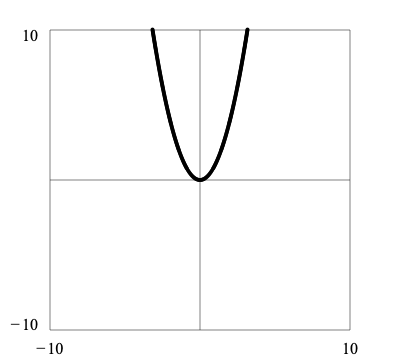
\includegraphics[scale=0.4]{parabola1.png}
\end{center}

The vectors \verb$xrange$ and \verb$yrange$ control the scale of the graph.

{\color{blue}
\begin{verbatim}
xrange = (-1,1)
yrange = (0,2)
draw(x^2)
\end{verbatim}}

\begin{center}
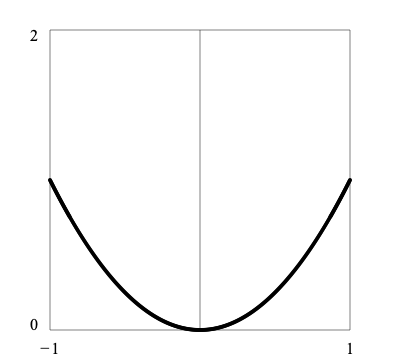
\includegraphics[scale=0.4]{parabola2.png}
\end{center}

Parametric drawing occurs when a function returns a vector.
The vector \verb$trange$ controls the parametric range.
The default is \verb$trange=(-pi,pi)$.
In the following example, \verb$draw$ varies \verb$theta$
over the default range $-\pi$ to $+\pi$.

{\color{blue}
\begin{verbatim}
xrange = (-10,10)
yrange = (-10,10)
f = 5 (cos(theta),sin(theta))
draw(f,theta)
\end{verbatim}}

\begin{center}
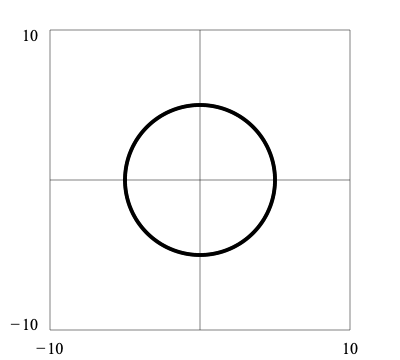
\includegraphics[scale=0.4]{circle1.png}
\end{center}

In the following example, \verb$trange$ is reduced
to draw a quarter circle instead of a full circle.

{\color{blue}
\begin{verbatim}
trange = (0,pi/2)
f = 5 (cos(theta),sin(theta))
draw(f,theta)
\end{verbatim}}

\begin{center}
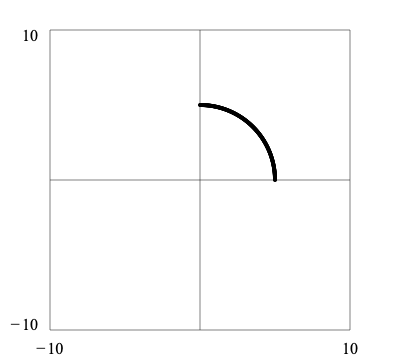
\includegraphics[scale=0.4]{circle2.png}
\end{center}

Draw a lemniscate.

{\color{blue}
\begin{verbatim}
trange = (-pi,pi)
X = cos(t) / (1 + sin(t)^2)
Y = sin(t) cos(t) / (1 + sin(t)^2)
f = 5 (X,Y)
draw(f,t)
\end{verbatim}}

\begin{center}
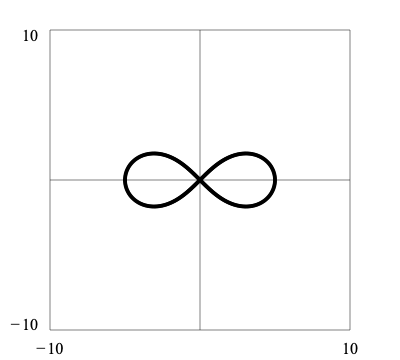
\includegraphics[scale=0.4]{lemniscate.png}
\end{center}

Draw a cardioid.

{\color{blue}
\begin{verbatim}
r = (1 + cos(t)) / 2
u = (cos(t),sin(t))
f = r u
xrange = (-1,1)
yrange = (-1,1)
trange = (0,2pi)
draw(f,t)
\end{verbatim}}

\begin{center}
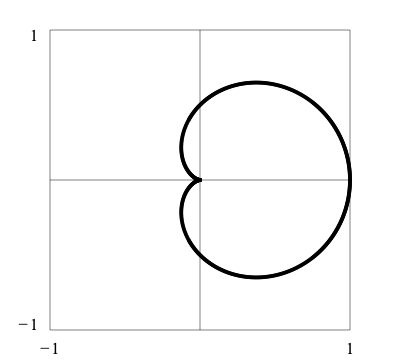
\includegraphics[scale=0.4]{cardioid.png}
\end{center}

\end{document}
